% Copyright 2019 Clara Eleonore Pavillet

% Author: Clara Eleonore Pavillet
% Description: This is an unofficial Oxford University Beamer Template I made from scratch. Feel free to use it, modify it, share it.
% Version: 1.0

\documentclass{beamer}
\usepackage{pdfpages}
% Load Packages
\usepackage[utf8]{inputenc}
\usepackage{xcolor}
\usepackage{tikz}
\usetikzlibrary{positioning,calc}
\usepackage{graphicx}
\usepackage{hyperref}
\usepackage{amsmath}
\usepackage{listings}
\usepackage{fontawesome}
\usepackage[T2A]{fontenc}
\usepackage[utf8]{inputenc}
\usepackage[russian]{babel}

% Define Commands
\newcommand*{\ClipSep}{0.06cm} %To adjust footer logo
\newcommand{\E}{\mathrm{e}\,} %\def\I{e} % used to defined e for exp(x), see later what it should be
\newcommand{\ud}{\mathrm{d}}
\lstset{numbers=left, numberstyle=\tiny, stepnumber=1,firstnumber=1,breaklines=true,
    numbersep=5pt,language=Python,
    stringstyle=\ttfamily,
    basicstyle=\footnotesize, 
    showstringspaces=false
}

\usetheme{oxonian}
\usepackage{wrapfig}
\usepackage{verbatim}
\usepackage{listings}

\title{OpenMP. Контролна работа 1.}
\subtitle{\textit{Курс „Паралелно програмиране“}}
\titlegraphic{{
\includegraphics[width=5.3cm]{iaps.png}}} 

\author{\newline \newline Стоян Мишев}

\vspace{1cm}

\date{} %\today

\begin{document}
\lstset{language=Python}
{\setbeamertemplate{footline}{} 
\frame{\titlepage}}


%%%%%%%%%%%%%%%%%%%%%%%%%%%%%%%%%%%%%%%%%%%%%%%%%%%

\begin{frame}
  \frametitle{Задача}
  Използвайки разгледания код от последното занятие, както и фрагмента от слайд 9,
  определете динамиката на системата от частици с данните от
  \url{https://hpc-old.cineca.it/content/exercise-5-0}. В частност,
  определете местоположението на частиците след 5 времеви интервала.

  В moodle качете файл с местоположенията на частиците в последния момент, както и написания от Вас код.
  
  Помислете дали е нужен \texttt{atomic} при обновяването на \texttt{pos} и \texttt{v}.

  --

  По желание, може да анимирате измененията в местоположенията на частиците.
\end{frame}

\begin{frame}{Помощни части от вариант на решение}
  
\includegraphics[width=0.8\textwidth]{help1}

  
\includegraphics[width=\textwidth]{help2}

  
\includegraphics[width=0.75\textwidth]{help3}

  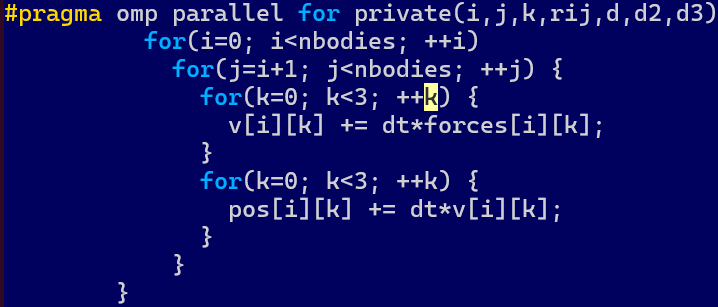
\includegraphics[width=0.7\textwidth]{help4}
\end{frame}

\end{document}


%%% Local Variables:
%%% mode: latex
%%% TeX-master: t
%%% End:

